% ---
% Capitulo de revisão de literatura
% ---
\chapter{Referencial Teórico}\label{cap:referencial_teorico}

\section{Realidade Aumentada}
	\citeonline{kirner2005aplicaccoes} explicam que a realidade aumentada é uma especificação de uma parte maior que é denominada realidade misturada, a realidade aumentada consiste primordialmente na sobreposição de imagens tridimensionais em ambientes reais e que podem ser vistas através de dispositivos computacionais como celulares ou computadores com acesso a câmeras. 
	
	A realidade aumentada pode ser definida ainda como o enriquecimento e melhoria de um ambiente do mundo real com texto, imagens e objetos virtuais sendo mostrados em tempo real através de um dispositivo computacional \cite{kirner2007realidade}.
	
	Segundo \citeonline{zorzal2006realidade}, O ambiente de realidade aumentada permite com que o usuário da aplicação interaja com os objetos virtuais introduzidos no ambiente real, sem que seja necessário o uso do equipamento extras como roupas, luvas e botas especiais.
	
	Para \citeonline{lindemann2014desenvolvimento}, a Realidade aumentada tem a capacidade e abrangência para impactar  quase todas as áreas da indústria, como militar, esporte, jogos, entretenimento, educação, negócios e por fim a área militar. Um dos campos que vem sendo bastante pesquisado a RA e com um grande potencial é a medicina, onde torna mais fácil a detecção de detalhes que são mais difíceis de ver a olho nú.
	
	\citeonline{desistemas} explicam que a Realidade Aumentada pode ser vista como uma integração entre informações virtuais como modelos 2D, 3D, imagens, áudio, vídeo e outros a visualizações do mundo real, onde tem características como:  
	\begin{itemize}
		\item Combinação do real com virtual;
		\item interação entre processos em tempo real;
		\item é mostrada em 3D;
	\end{itemize}
	
	Segundo \citeonline{fraga2017ambiente}, A Realidade virtual é a definição de um sistema que principalmente sintético, porem contem algumas imagens do mundo real, sendo com isso possível a criação por exemplo de um ambiente de aprendizagem híbrido e imersivo, para facilitar o desenvolvimento de habilidades nos alunos. 
	
	
	\begin{figure}[H]
		\centering
		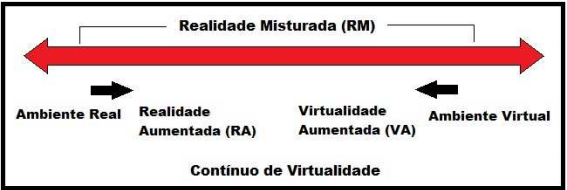
\includegraphics[scale=1]{imagens/misturada}
		\caption{Níveis de Realidade Misturada}
		Fonte: \citeonline{rovadosky2012aplicaccao}
		\label{fig:misturada}
	\end{figure}
	
	A Figura \ref{fig:misturada}, é uma proposta de \citeonline{rovadosky2012aplicaccao}, onde é mostrado que a RA faz parte de um conjunto, chamado de realidade aumentada, sendo que ela está mais para o uso em ambiente real do que a realidade virtual, que está mais voltada ao ambiente totalmente virtualizado.

	\begin{figure}[H]
		\centering
		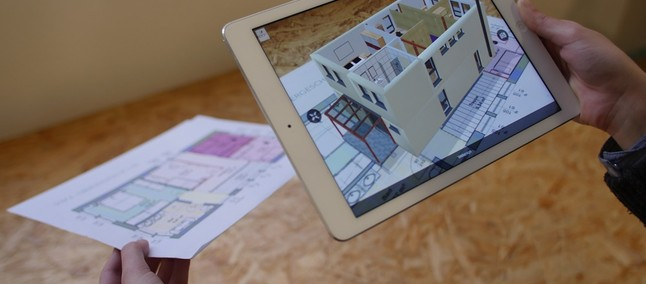
\includegraphics[scale=0.7]{imagens/raarqui}
		\caption{Demonstração de RA na Arquitetura}
		Fonte: Tudo Celular, 2018
		\label{fig:arquitetura}
	\end{figure}
	
	A Figura \ref{fig:arquitetura} mostra o uso da realidade aumentada na área da arquitetura e engenharia, demonstrando assim que essa tecnologia se faz útil pela facilidade que ela traz na visualização de algo que ainda não é concreto ou palpável.
	
	
\section{Geolocalização}
	Segundo \citeonline{carvalho2017potencia}, a geolocalização se tornou possível e acessível após os seus criadores, ou seja, o departamento de defesa dos Estados Unidos da América, liberar aos civis. Esta tecnologia começou a ser desenvolvida no ano de 1972 e tinha como objetivo ser uma tecnologia apenas de auxilio militar.
	
	O aparelho de GPS tem a função de enviar sinais para os satélites, dessa maneira fazendo os cálculos da localização, onde tem-se ao todo cinco estações espalhadas ao redor do globo terrestre onde essas tem a função de atualizar  e sincronizar a posição dos satélites e dos relógios atômicos que se encontram dentro dos mesmos \cite{gps:tecmundo}.
	
	Para \citeonline{santos2015desenvolvimento}, a geolocalização se trata da arte de descobrir onde se encontra um determinado usuário, por meio de suas coordenadas, e dar como opção o compartilhamento dessas informações por meio de aplicativos web ou mobile. Sendo que os primeiros métodos de descoberta era baseado na localização do IP do dispositivo, o que era pouco confiável.
	
	\citeonline{costa2012desenvolvimento}, explica que o georreferenciamento se dar pela triangulação das torres que dão cobertura telefônica aquele aparelho, trabalhando em conjunto com satélites de GPS, com isso é possível ter a localização em tempo real do dispositivo.
	
	\begin{figure}[H]
		\centering
		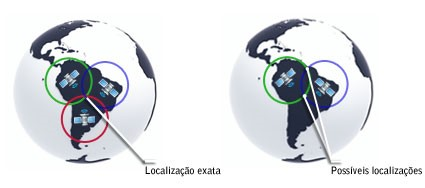
\includegraphics[scale=1]{imagens/triangulacao}
		\caption{Triangulação Via GPS e Torres}
		Fonte: Tecmundo, 2009
		\label{fig:triangulacao}
	\end{figure}
	
	A Figura \ref{fig:triangulacao} mostra a triangulação das torres e a ação dos satélites para determinar a localização dos dispositivos, na qual no pior caso é possível a localização de possíveis pontos onde o usuário está e na melhor das opções é dada a localização exata do ponto.
	\subsection{Google Maps}
		\citeonline{neto2014desenvolvimento} explicam que o google maps é uma biblioteca lançada pela google no ano de 2005 que permite a criação de aplicações mobile e web por meio de APIs que são distribuídas de forma gratuita e funcionando em âmbito global, onde é possível a visualização da localização em camadas como ruas, imagens de satélite e também de forma hibrida, mesclando as duas anteriores.
		\begin{figure}[H]
			\centering
			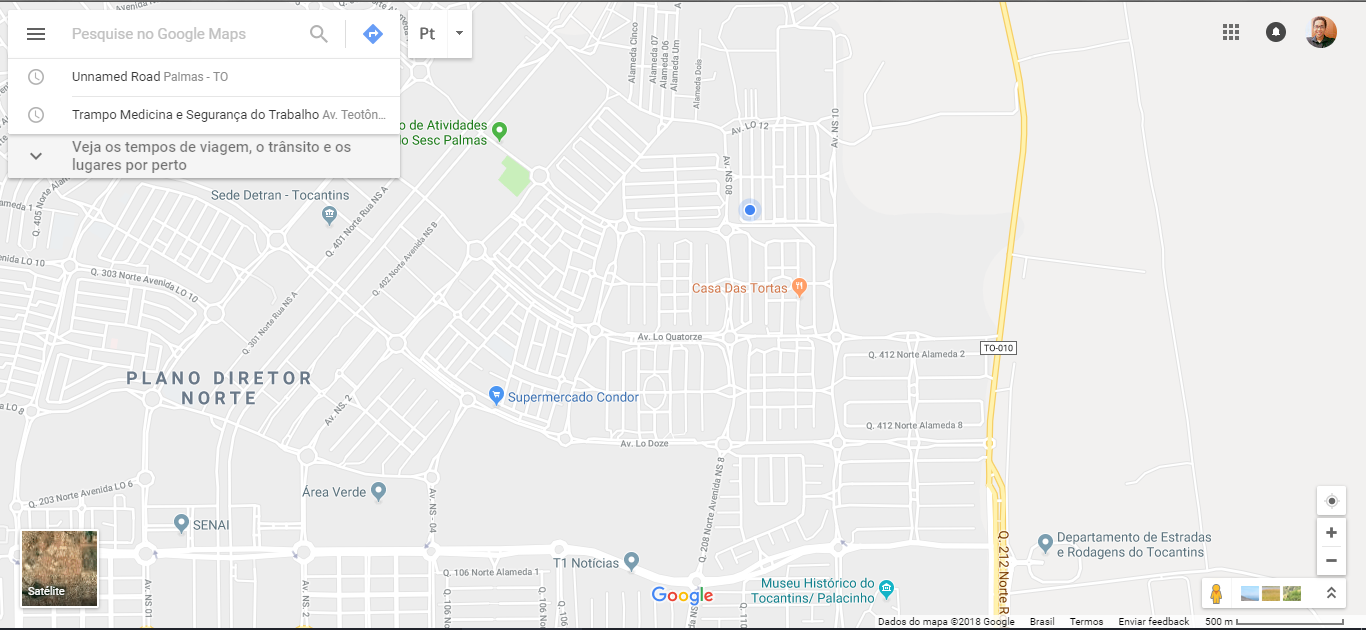
\includegraphics[scale=0.4]{imagens/gmaps}
			\caption{Localização via Google Maps}
			Fonte: Google, 2018
			\label{fig:gmaps}
		\end{figure}
		A Figura \ref{fig:gmaps} mostra a localização em que se encontra o dispositivo que realizou a captura, sendo essa  obtida através do conhecimento do posicionamento georográfico em que se encontra o dispositivo.
		
	\subsection{Waze}
	Segundo \citeonline{faria2014vamos}, a Waze surgiu no ano de 2008 quando um dos fundadores, o engenheiro Ehud Shabtai ao receber um aparelho de GPS percebe que o seus mapas estão todos desatualizado, com isso ele reuniu um grupo de amigos para resolver o problema, eles hackearam o sistema do GPS e corrigiram as falhas, inserindo assim os mapas que faltavam. Com o ocorrido a empresa detentora dos direitos do aparelho e fabricante resolveu emitir um documento informando que eles não teriam permissão para tal alteração e tinham cometido uma infração ao alterar o aparelho de GPS, com isso Ehud Shabtai e seus companheiros decidem criar o próprio sistema de geolocalização deles, assim surge o aplicativo onde os próprios usuários podem ajudar a montar os mapas, o Waze.
	
	\begin{figure}[H]
		\centering
		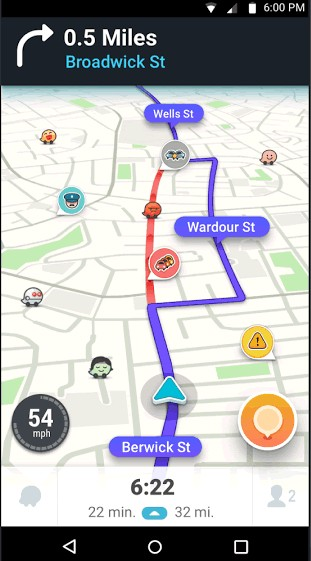
\includegraphics[scale=0.4]{imagens/waze}
		\caption{Localização via Waze}
		Fonte: Waze, 2018
		\label{fig:waze}	
	\end{figure}

		A Figura \ref{fig:waze} mostra o funcionamento do aplicativo de geolocalização Waze, onde é possivel a costumização de pinos em locais, a voz do narrador de caminho, ou seja, é possível o usuário deixar o app como ele desejar.
	
\section{Bibliotecas Destinadas ao Desenvolvimento de Aplicativos com RA e Geolocalização}

	\subsection{ARToolKit}
		\citeonline{francca:2005} explicam que o ARToolKit é uma biblioteca usada para o desenvolvimento de aplicações baseadas em realidade aumentada, fazendo o uso de visão computacional para realização de  cálculos sobre um conjunto de marcadores com relação ao ambiente capturado pela câmera do dispositivo para com essas informações poder inserir objetos 3D à aquele ambiente.
		
		%Linguagem
		Segundo \citeonline{hitl:2000}, o ARToolKit é uma biblioteca escrita em linguagem C e C++ que permite a fácil criação de aplicativo baseados em Realidade aumentada, que se consiste na sobreposição de imagens virtuais feitas por computação gráfica ao mundo real.
		
		\begin{figure}[H]
			\centering
			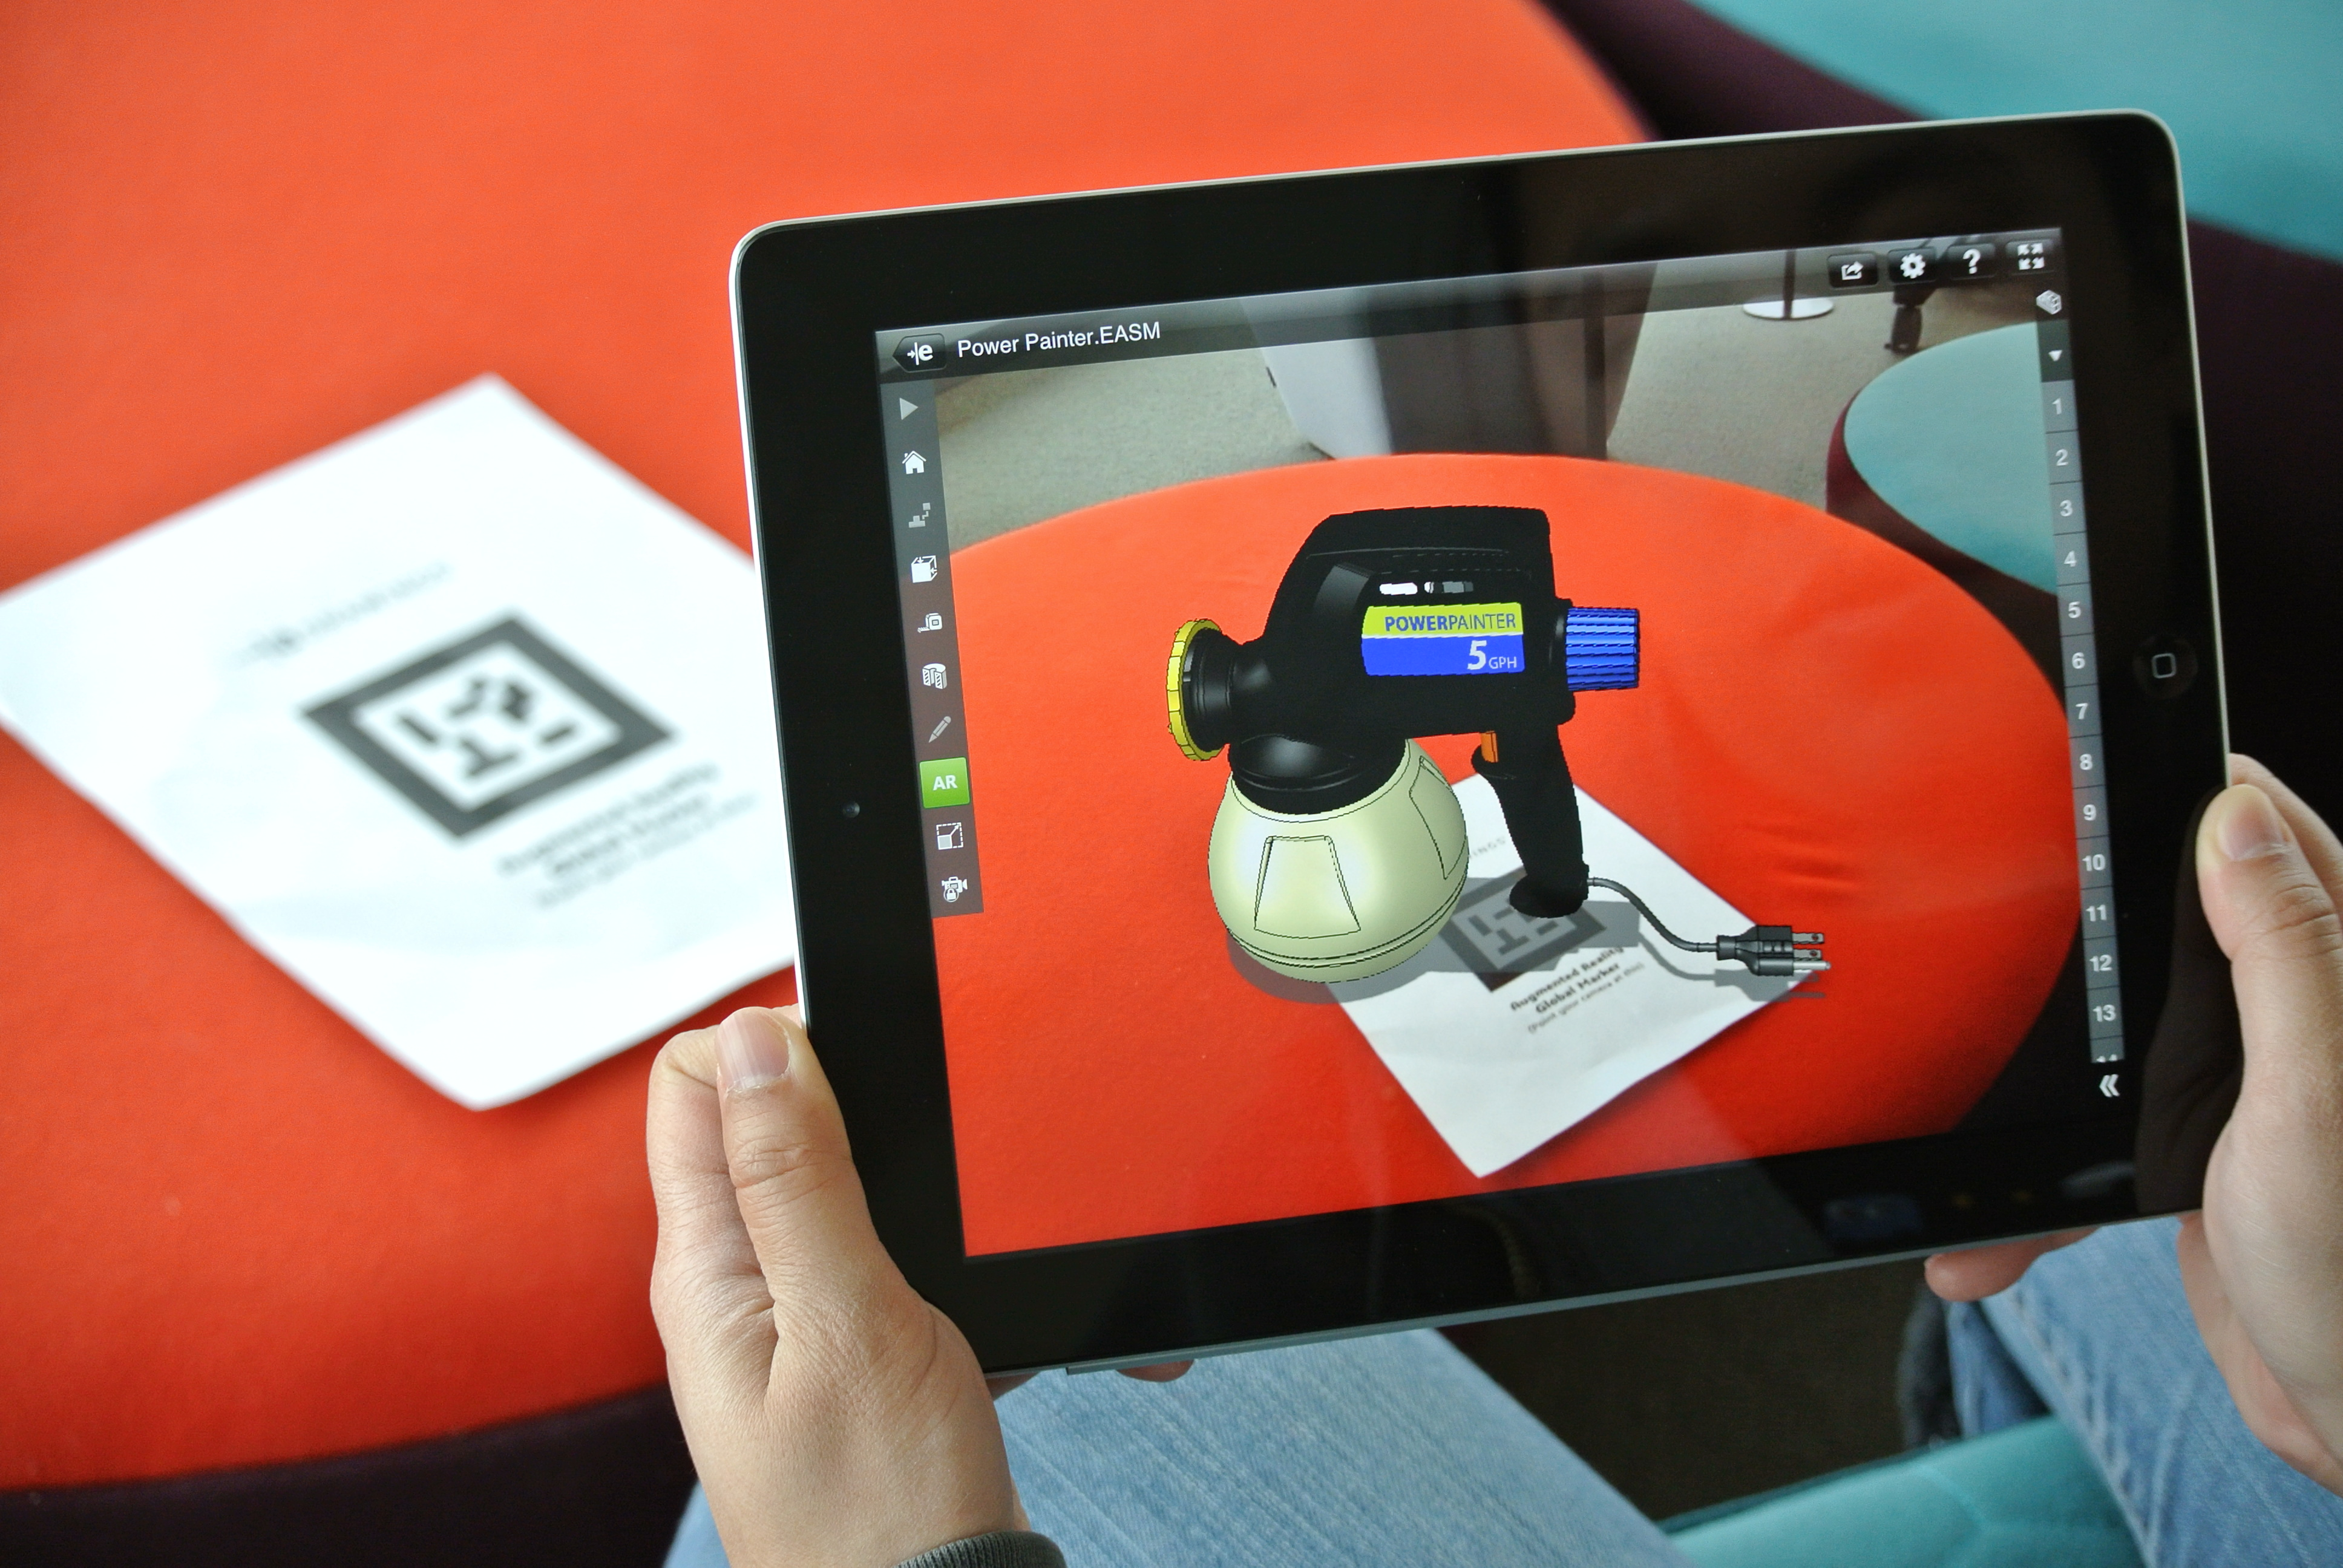
\includegraphics[scale=0.4]{imagens/artoolkit}
			\caption{Imagem 3D a partir de Ancore ARtoolKit}
			Fonte: Emerce, 2017
			\label{fig:artoolkit}
		\end{figure}
		
		%plataforma de execução
		O código fonte do ARtoolKit se encontra disponível na página deles no repositório github, sendo assim o mesmo é um software livre e também \textit{open-source}, o que implica no fato de poder ser alterado por quem desejar ajudar no projeto e está disponível para a criação de aplicações para as plataforma Mac OS e iOS da Apple e também para computadores com \textit{windows} ou linux e dispositivos móveis com sistema operacional android \cite{faganholi}.
	\subsection{Vuforia}
		\citeonline{ibanez:2013} explicam que o vulforia  é uma sdk de realidade aumentada para \textit{smarthphones}, que utiliza técnicas de visão computacional para fazer o reconhecimento e rastreio de objetos virtuais pela câmera do dispositivo no ambiente real, sendo ainda capaz de suportar tanto imagens virtuais em 3D quanto 2D e essas aplicações podem ser feitas nativamente tanto para os sistema operacional Android quanto para iOs por meio da \textit{game engine Unity}.
		
		%Linguagem	
		Segundo \citeonline{more:2016}, o Vuforia se trata de uma \textit{engine} criada pela \textit{Qualcomm Developer Network}, que serve para a criação de objetos em realidade aumentada para ser utilizada no desenvolvimento de aplicativos de dispositivos móveis, sendo bastante utilizada nas linguagens C++, Java e .Net.
		
		O Kit de desenvolvimento de software SDK Vuforia permite o  desenvolvimento de aplicações de ralidade aumentada a partir de imagens que são chamadas de marcadores, sendo que o mesmo tem suporte as plataformas Android, iOs e também unity, O vuforia ainda permite que seja criado um banco de dados contendo os marcadores, sendo possível o envio e armazenamento de até mil marcadores de objetos virtuais \cite{bergamaschi2014estudo}.
		
		\begin{figure}[H]
			\centering
			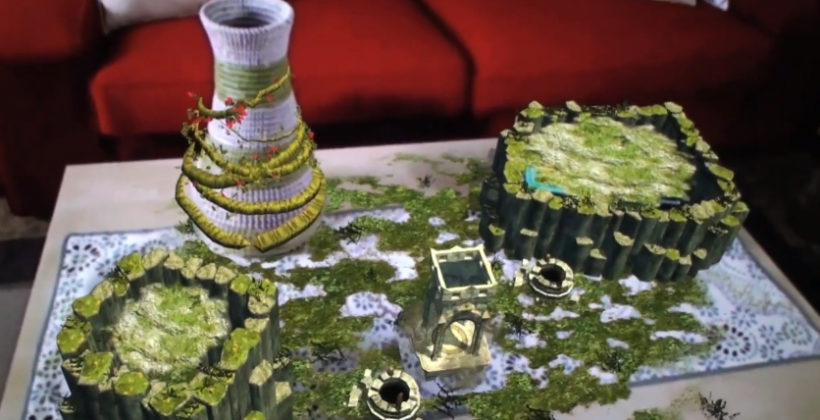
\includegraphics[scale=0.5]{imagens/vuforia-jogo}
			\caption{Demononstração Jogo RA Vuforia}
			Fonte: Qualcomm, 2018
			\label{fig:vuforia-jogo}
		\end{figure}
		
		Para uso do vuforia no desenvolvimento de aplicação é preciso pagar um plano de assinatura, onde tem plano \textit{Clound} com pagamento mensal, que custa \$ 99 dólares e pode usufruir de diversos benefícios oferecidos pela plataformas ou pode-se optar pelo plano \textit{Classic} que custa um total de \$ 499 dólares e é pago somente uma vez, porém o numero de recurso é reduzido e por fim, tem-se o plano Pro, onde o preço é dado dependendo do rendimento da empresa, é requerido por empresas com rendimento superior a 10 milhões por ano \cite{vuforia:2018}.
		
		
	\subsection{LayAR}
		Segundo \citeonline{manzano:2016}, o LayAR se trata de um software usado para criar e/ou editar conteúdos de realidade aumentada, que tem as áreas de publicidade, arquitetura e turismo como maiores interessado e que fazem o seu uso, a empresa responsável foi fundada no ano de 2009, e no inicio do ano de 2016 já contava com um total de mais de 500 mil páginas com conteúdo em realidade aumentada.
		
		\citeonline{de:2014} explicam que o LayAR funciona sobrepondo imagens, que são conhecidas como PI's do usuário, sendo eles exibidos na tela do usuário de duas formas, são elas: um disco sólido maciço, colorido e com um ícone ou um modelo 3D, onde clicando neles é possível obter mais informações sobre o objeto virtual.
		
		%Custo
		O LayAR oferece dois planos pra quem deseja desenvolver aplicativos de realidade aumentada para publicar nas lojas, o primeiro é o básico onde tem um preço de \$ 15,90 dólares e o desenvolvedor tem disponível botões básicos, botões de mídias e de redes sociais e ainda inclui a hospedagem de vídeos que serão exibidos na aplicação, eles também oferecem um plano de \$ 79 dólares onde inclui as mesma vantagens que o plano anterior e algumas outras como estatísticas \cite{layar:2018}.
	\subsection{ARCore}
		O ARCore se trata de uma plataforma desenvolvida pela google para o desenvolvimento de aplicações voltadas a realidade aumentada, com as diferentes API's que nela existe é possível fazer com que o dispositivo realize ações como: detecção do ambiente em que se encontra, compreender as características do espaço e a interação entre os objetos virtuais e o usuário \cite{google:2018}.
		
		\begin{figure}[H]
			\centering
			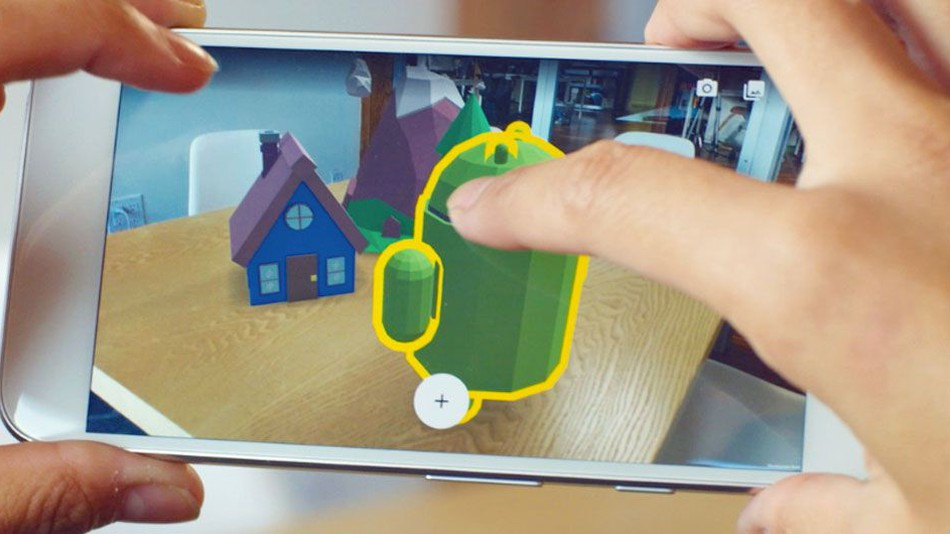
\includegraphics[scale=0.4]{imagens/arcore}
			\caption{Demonstração do Funcionamento do ARCore}
			Fonte: Google, 2018
			\label{fig:arcore}
		\end{figure}
		
		\citeonline{correiadev} explicam que o ARCore usa-se de três tecnologias para fazer a interação dos objetos gerados virtualmente com o mundo real, sendo elas: 
			\begin{itemize}
				\item O rastreamento da posição do dispositivo com relação ao mundo real.
				\item A compreensão do ambiente para detectar como é a superfície que será colocado o objeto virtual. 
				\item E a estimativa de luz, que permite o objeto interagir com a luz do ambiente em que ele se encontra.
			\end{itemize} 
		
		%Plataformas de desenvolvimento
		Segundo a \citeonline{google:2018}, O ARCore fornece um SDK para diferentes plataformas de desenvolvimento, como por exemplo \textit{Unity Engine}, \textit{Unreal}, Android Studio e inclusive para sistemas operacional da Apple iOs.
		
		%Plataforma de execurção
		O ARCore requer que os aparelhos cumpram alguns requisito para que seja executada uma aplicação AR, sendo esse requisitos alguns modelos de celular com android na versão 7 ou superior, dispositivo que venha de fábrica com uma instalação da \textit{Google play store} e por fim o \textit{OpenGL} na versão 3.0, a lista de dispositivos é bastante curta, mas a google afirma que está em contato com as fabricantes para que se expanda a quantidade de aparelhos que rodam ARCore \cite{google:2018}.

\section{Artigos e Trabalhos Relacionados}	

	\subsection{Pokémon GO}
	Segundo dados da empresa criadora do jogo, \citeonline{niantic:2018}, após o lançamento do mesmo em julho de 2016 o sucesso foi imediato, de modo que o jogo se tornou o aplicativo de realidade aumentada mais usado e rentável de todos os tempos. A empresa se orgulha ainda do fato de nos dois primeiros meses todos os jogadores juntos percorreram cerca de 4,6 milhões de quilômetros e após três meses essa distância aumentou para 8,7 milhões de quilômetros percorridos.
	
	\citeonline{wagner:2017} definem o jogo Pokémon GO, como um jogo que permite o usuário procurar criaturas fictícias, do universo da franquia Pokémon, com o uso de recursos do celular como a geolocalização e a realidade aumentada, que se trata de componentes virtuais inseridas no ambiente real, para isso o jogador precisa se mover no mundo real e assim realizar as captura.Sendo que o jogador pode tomar ações como, fazer com que seus pokémom lutem contra os de outros jogadores, chocar ovos de acordo com a quilometragem percorrida, conquistar ginásios por batalhas e pegar itens em paradas que são chamadas de pokestops. 
	
	\begin{figure}[H]
		\centering
		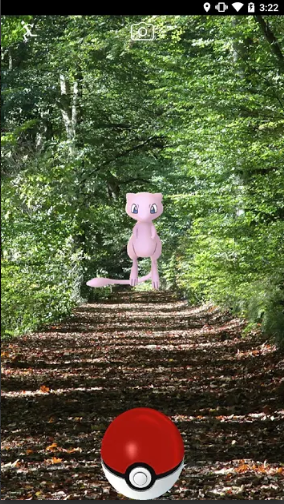
\includegraphics[scale=0.6]{imagens/pokemongo}
		\caption{Captura de Pokémon}
		Fonte: Niantic, 2018
		\label{fig:pokemongo}
	\end{figure}
	
	A \citeonline{niantic:2018} cita ainda que a arrecadação com o jogo no final de 2016 chegou a marca de 1 bilhão de dólares e no ano de 2017 o jogo chegou a marca de 650 milhões de \textit{downloads} e todos os jogadores andaram juntos um total de 15,8 bilhões de quilômetros, no inicio do ano de 2018 o jogo já havia superado a marca de 800 milhões de \textit{downloads}.
	
	A Figura \ref{fig:pokemongo} mostra o funcionamento do jogo, onde pela câmera do celular é possível enxergar os elementos do jogo, como o Pokémon e a pokébola que será utilizada para captura-lo aparecendo no ambiente do mundo real onde o jogador se encontra.
	
	\subsection{Ingress}
	Segundo a \citeonline{niantic:2018} que é a produtora do jogo, afirma que ele foi o primeiro jogo de realidade aumentada para \textit{smartphones}, lançado em novembro de 2012, onde é feito o uso de geolocalização e o mundo real é usado como o campo de jogo.
	
	A mecânica do jogo consiste em o jogador chegar a locais chamados de portais, onde são encontrados os principais recursos do jogo, a matéria exótica, esse elemento é usado para realizar todas as ações do jogo. No inicio o jogador deve fazer a escolha de uma equipe da qual fará parte, sendo elas: A resistência, que se trata de uma equipe que procura lutar contra força que buscam usar a matéria exótica para a escravização da humanidade e a outra equipe são os iluminados, que busca usar o poder da matéria escura para evoluir a humanidade \cite{sobke:2017}.
	
	\begin{figure}[H]
		\centering
		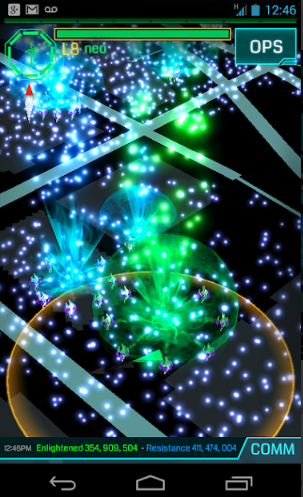
\includegraphics[scale=0.6]{imagens/ingress}
		\caption{Portal de Matéria Escura}
		Fonte: Niantic, 2018
		\label{fig:ingress}
	\end{figure}
	
	A Figura \ref{fig:ingress} mostra os portais de matéria exótica que aparecem no jogo que estão em uma localizações do mundo real, onde o jogador precisa ir até elas para fazer a coleta e também ver através do recurso de realidade aumentada os portais.
	
	\subsection{ZAP Explora}
	Segundo a \citeonline{zap:2017} o aplicativo consiste em uma forma de o usuário poder ver informações de imóveis para aluguel ou venda como preço, valor de IPTU, quantidades de cômodos, fotos, descrição e diversas outras informações importantes, porém o diferencial é que esses dados podem ser vistas apenas apontando a câmera do celular para uma determinada direção ou imóvel, dessa forma, será mostrado um quadro clicável contendo as informações e formas de contato com o dono, a aplicação é da zap imóveis e com isso terá apenas imóveis que estão disponíveis por meio da mesma empresa.
	
	\begin{figure}[H]
		\centering
		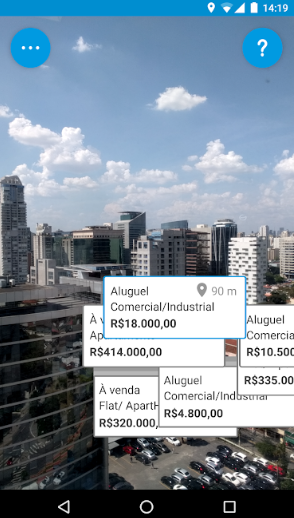
\includegraphics[scale=0.6]{imagens/zapexplora}
		\caption{Demonstração do Zap Explora}
		Fonte: ZAP Imóveis, 2018
		\label{fig:zap} 
	\end{figure}
	
	A Figura \ref{fig:zap} mostra a forma como o aplicativo funciona, com a câmera posicionada para um determinado local os imóveis que estão disponíveis para venda ou aluguel naquela região pela zap imóveis são mostrados e com isso o usuário poderá ter mais informações sobre o local de maneira bem mais confortável e dinâmica.
	
	\subsection{Pinmyspot}
	\citeonline{schenkel:2018} explica que o Pinmyspot é um jogo de realidade aumentada em conjunto com geolocalização em que é preciso que o jogador sair em busca de pins que darão a ele descontos em diversos tipos de produtos. Ainda segundo a empresa que produz o jogo  já foram contabilizados mais de 40 mil capturas de descontos e o jogo chegou a ser baixado mais de 50 mil vezes nas lojas de aplicativos.
	
	Segundo \citeonline{startupsstars} o Pinmyspot se trata de uma rede social gamificada,que mistura tecnologias de geolocalização e realidade aumentada, que além de ter a opção de conseguir descontos os usuários podem ver e deixar fotos em realidade aumentada no local escolhido, podendo assim ser visto por outros usuários, sendo em forma privada, ou seja, somente quem é marcado pode ver, ou de forma pública, todos que que usam o aplicativo e passarem por aquele local podem ver as fotos.
	
	\begin{figure}[H]
		\centering
		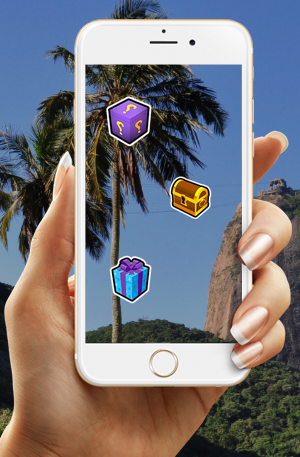
\includegraphics[scale=0.7]{imagens/pinmyspot}
		\caption{Demonstração do Pinmyspot}
		Fonte: Pinmyspot, 2018
		\label{fig:pinmyspt} 
	\end{figure}
	
	A Figura \ref{fig:pinmyspt}, mostra o app em execução, onde o usuário apontando a câmera do celular é possível a visualização de descontos, presentes ou até mesmo fotos que as pessoas que já passaram por aquele local deixou.
	
	\subsection{FlirtAR}
	A \citeonline{Cawley:2017} explica que o FlirtAR se trata de um aplicativo disponível para as plataformas Android e iOs que usa a tecnologia de realidade aumentada e geolocalização onde de acordo com a direção em que seu usuários aponta a câmera são mostradas informações sobre outras pessoas que usam o aplicativo, dessa maneira é possível que a pessoa em posse do aplicativo possa escolher um pretendente de acordo com essas características apresentadas.O fato de ser preciso está no local para poder ver informações de outros usuários faz com que haja a possibilidade de um encontro imediato. A partir do aplicativo é possível fazer os cálculos da compatibilidade que há entre as duas pessoas envolvidas.
	
	A empresa que leva o nome do aplicativo foi fundado em 2017 pelo Brasileiro Renan Godinho, que na época tinha 26 anos de idade, e dizia que as pessoas passam muitas horas em aplicativos de relacionamentos escolhendo pretendentes e geralmente nunca os encontram, e quando consegue encontrar muitas vezes as pessoas envolvidas não combinam. O desenvolvimento do aplicativo foi iniciado em março de 2017 e teve seu lançamento dia 30 de setembro de 2017 para a plataforma iOs e 30 de outubro de 2017 para a plataforma Android \cite{chloe:2017}.
	
	\begin{figure}[H]
		\centering
		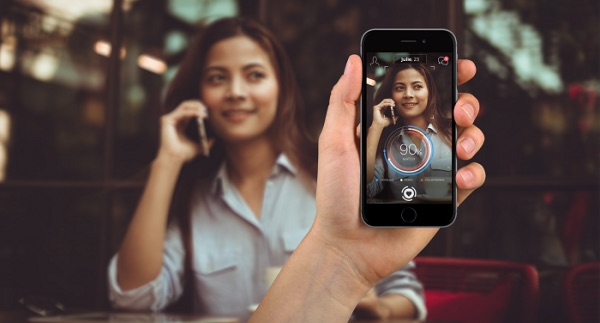
\includegraphics[scale=0.4]{imagens/flirtar}
		\caption{Demonstração do FlirtAR}
		Fonte: FlirtAR, 2018
		\label{fig:flirtar}
	\end{figure}
	
	A Figura \ref{fig:flirtar} mostra a representação de funcionamento do aplicativo, onde em meio a uma multidão ao usuário apontar a câmera é possível ver perfil de outras pessoas que estão naquele lugar e que usam o aplicativo.
	\subsection{Geocaching}
	O \textit{Geocaching} é um jogo de realidade aumentada lançado no ano de 2000, onde chegou a ter um um total de 2,4 milhões de localizações salvas e mais de 6 milhões de jogadores ativos, na qual pode-se notar a junção de elementos como a tecnologia e uma brincadeira bastante conhecida que é a caça ao tesouro. \cite{2014geocaching}.
	
	\citeonline{alencar2011} explica que tudo começou com Dave Ulmer, que após os Estados Unidos da América liberar acesso ao GPS pelos civis,teve a ideia de esconder um pacote em Portland, no estado de Oregon, e com isso registrou a localização desse pacote em um site, com isso outro usuário do site viu a localização e foi atrás do pacote e o encontrou, marcando que esteve naquela localização para que outros usuários pudessem saber que o pacote foi encontrado, surgindo assim o \textit{Geocaching}.
	
	Segundo o site oficial do projeto \citeonline{geocaching:2018}, atualmente existem um total de 3 milhões de jogadores ativos que são chamados de \textit{geocaches} e estão espalhados por 190 países diferentes em todo o mundo.
	
	
	\begin{figure}[H]
		\centering
		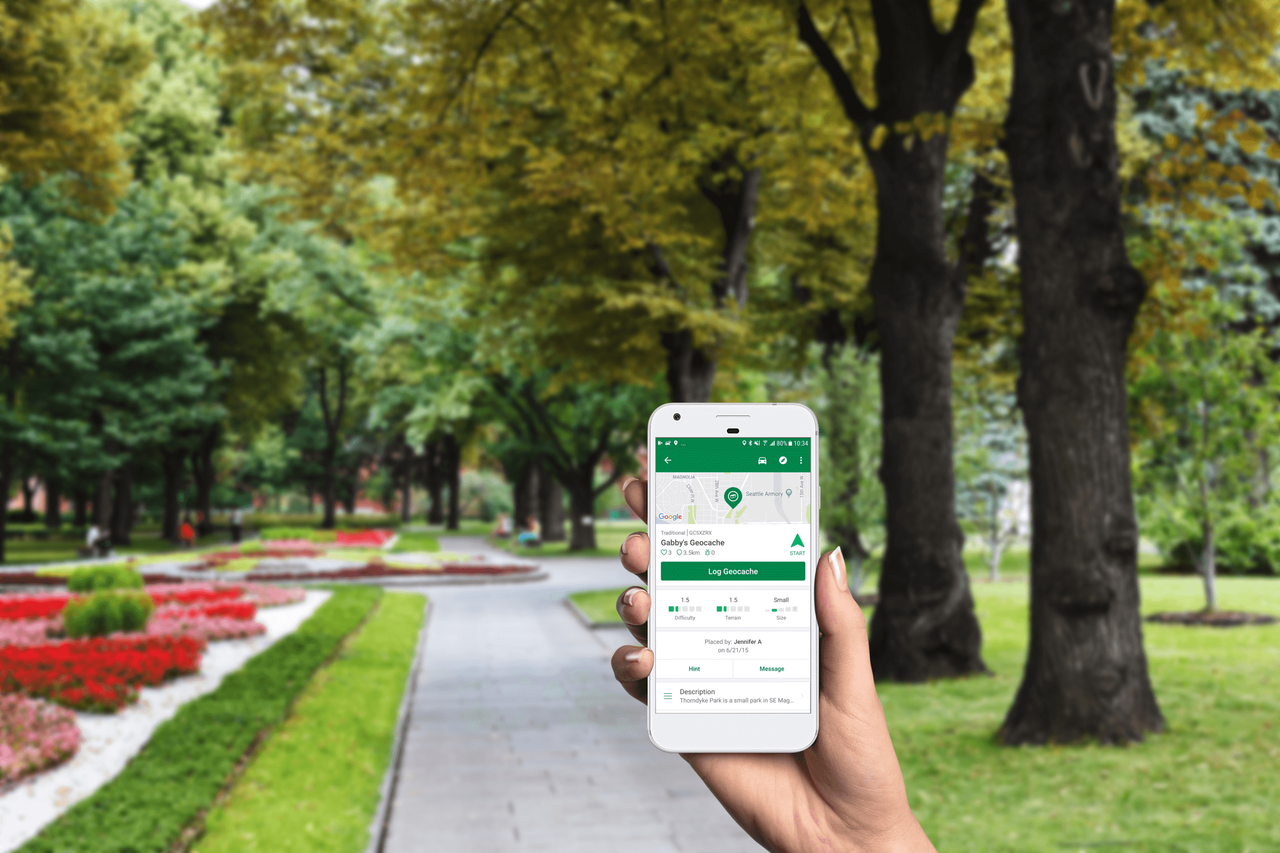
\includegraphics[scale=0.3]{imagens/geocaching}
		\caption{Demonstração do Geocaching}
		Fonte: Geocaching, 2018
		\label{fig:geocahing}
	\end{figure}
	
	\citeonline{alencar2011} traz algumas regras para as pessoas que pretendem começar essa aventura, como: Ter uma conta registrada no site, saber como é o funcionamento do GPS, selecionar um cache a partir da dificuldade do terreno em que a pessoa se encontra, esconder o cache e registrar sua localização no aplicativo e por fim sair para descobrir novos caches.
	
	A Figura \ref{fig:geocahing} é uma simulação de como funciona o aplicativo, onde os pacotes aparecem em uma determinada localização e o \textit{geocaching} é conduzido até lá por meio do aplicativo.
	\subsection{Jurassic World™ Alive}
	Segundo a \citeonline{universal:2018}, o jogo é uma parceria entre ela mesma que é a produtora da franquia de filmes e da Ludia Inc. que é um estúdio de desenvolvimento de games, e foi desenvolvido para ser lançado na mesma época que o filme \textit{Jurassic World: Fallen Kingdom} que teve sua estreia nos cinemas canadenses e estadunidense no dia 22 de julho de 2018.
	
	A \citeonline{ludia:2018}, explica que o jogo se baseia em cinco pilares, sendo eles:
	A Exploração do mundo real com o auxilio de geolocalização e realidade aumentada do celular, a Coleta de diferentes raças de dinossauros e materiais genéticos das criaturas, a criação de raças baseada nos materiais genéticos coletados, a Batalha podendo ser por convite em uma partida jogador versus jogador ou para se defender em uma eventual ameaça e por fim ganhar recompensas ao encontrar pontos que são chamados de \textit{Supply Drops}.
	
	
	\begin{figure}[H]
		\centering
		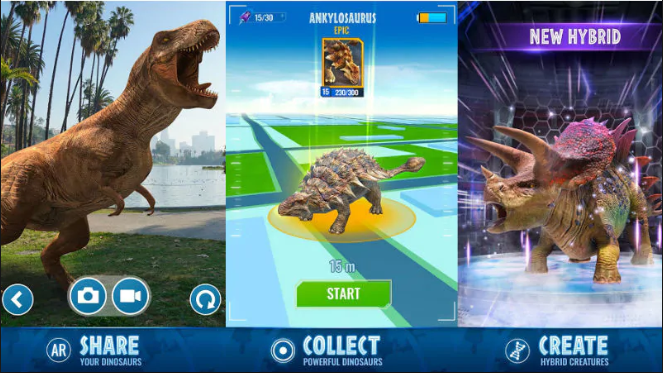
\includegraphics[scale=0.7]{imagens/jurassicword}
		\caption{Componentes do Jogo Jurassic Word Alive}
		Fonte: Ludia, 2018
		\label{fig:jurassicwordalive}
	\end{figure}
	A Figura \ref{fig:jurassicwordalive} mostra algumas formas de interação do jogo, onde na primeira é possível através da realidade aumentada "tirar fotos" dos dinossauros que o jogador tem para compartilhar, na segunda mostra o uso da geolocalização para mostrar onde estão os dinossauros a serem capturados e na terceira é possível ver o laboratório de criação de novas espécies.
	%\subsection{Ghostbusters World}
	\subsection{Guia Turístico em Dispositivo Móvel Baseado em Ra-Mobiguidetour}
		É um projeto apresentado por \citeonline{rodrigues2011guia}, que consiste em um ambiente computacional multimídia e interativo para a área de turismo que possa estar disponível através de um dispositivo móvel e que possibilite ao usuário expandir seu conhecimento sobre monumentos históricos, atrações turística e até chegando a substituir os panfletos de papel que são comuns.
		
		O Autor explica ainda que o ambiente foi desenvolvido pensando em pessoas que tem o costume de viajar muito e para diversos lugares diferentes e que gostam de aprender mais sobre onde visitam, pelo fato de o aplicativo fornecer diversas imagens e textos que o ajudam a entender sobre aquele lugar.
		
		O aplicativo é feito usando a biblioteca ARToolKit e funciona com marcadores grudados em cada um dos pontos turístico, onde o usuário vai escanear com a interface do aplicativo assim ele poderá ver informações sobre aquele determinado local ou monumento.  
		
		\begin{figure}[H]
			\centering
			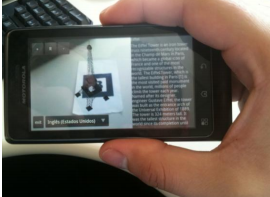
\includegraphics[scale=1]{imagens/MobiGuideTour}
			\caption{Funcionamento do MobiGuideTour}
			Fonte: \citeonline{rodrigues2011guia}
			\label{fig:mobiguide}
		\end{figure}
		
		A Figura \ref{fig:mobiguide} mostra a demonstração de funcionamento do aplicativo, onde o marcador contem as informações da torre Eiffel, e o usuário estando no local, e achando esse marcador, basta apontar a câmera do celular com o app que aparecerá todas as informações sobre aquele ponto.
		
	\subsection{Jogo Baseado na Localização para a Otimização da Experiência Turística}
		Segundo o autor do projeto, \citeonline{pereira2016jogo}, o objetivo é produzir um protótipo de jogo para as plataformas móveis, onde tem o objetivo de incentivar o turismo, sendo o projeto centrado em um parque de sua cidade, com informações de fauna e flora.
		
		Ainda segundo o autor do projeto, o  aplicativo funciona offline, porém a precisão dos dados aumenta se a mesma estiver ligada, o jogo possui um mapa do parque e através dele o jogador deve andar e procurar para desbloquear novas espécies de plantas e animais no jogo
		
		O jogo é composto também por diversos \textit{minigames}, onde vai ajudar o turista a conhecer melhor o local, e a biodiversidade que ali se encontra e ainda se divertindo no processo de aprendizado.
		
		\begin{figure}[H]
			\centering
			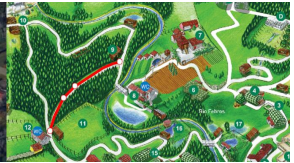
\includegraphics[scale=1]{imagens/parque}
			\caption{Mapa do Jogo de Turismo no Parque}
			Fonte: \citeonline{pereira2016jogo}
			\label{fig:parque}
		\end{figure}
		
		A Figura \ref{fig:parque}, mostra o o mapa que aparece no aplicativo de \citeonline{pereira2016jogo}, onde é tudo mapeado via geolocalização do celular, e é onde ocorre os \textit{MiniGames}.
	
	\subsection{Desenvolvimento de Aplicativo para Visualização de Patrimônio Histórico-Arquitetônico em Realidade Aumentada}
		O trabalho apresentado por \citeonline{silva2012desenvolvimento} tratam de um aplicativo que teve seu desenvolvimento baseado na linguagem \textit{ActionScript},e utilizou a versão para a linguagem da biblioteca ARToolKit, que se chama FLARToolKit, que funciona da mesma forma, com o reconhecimento de ancoras, e é direcionado para computadores com \textit{webcam}.
		
		O aplicativo funciona na web, através de um navegador de internet, sendo que o usuário precisa acessar o site da aplicação, e através do menu da aplicação o usuário deve escolher qual modelo de cartão com ancora está em sua posse, assim depois apontar a câmera do computador para o cartão e assim terá o objeto 3D, de algum local turístico.
		
		\begin{figure}[H]
			\centering
			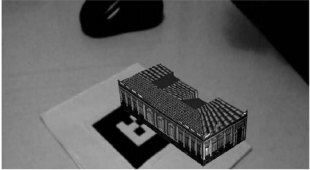
\includegraphics[scale=1]{imagens/arquitetura}
			\caption{Aplicativo de Visualização de Locais Arquitetônicos}
			Fonte: \citeonline{silva2012desenvolvimento}
			\label{fig:arq}
		\end{figure}
		
		A Figura \ref{fig:arq}, apresenta o modelo 3D de uma obra arquitetônica, que é apresentada através de um marcador do ARToolKit, e que é mostrado pelo navegador por meio do aplicativo. 
		 